\documentclass{article}
\usepackage{graphicx}
\usepackage{caption}
\graphicspath{ {./images/} }
 
\begin{document}
\paragraph{A first Look at the Captured Trace}
  \begin{enumerate}
    \item Select one UDP packet form your trace.  From this packet, determine how many fields there are in the UDP header.  Name these fields
        \begin{itemize}
          \item There are Four fields in the UDP Header:
            \begin{itemize}
              \item Source Port
              \item Destination Port
              \item Length
              \item Checksum
            \end{itemize}
          \item 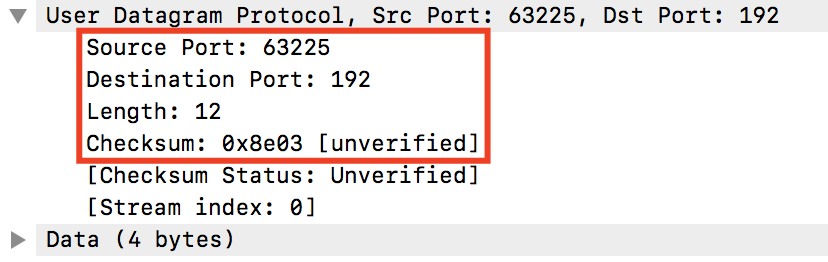
\includegraphics[scale=0.5]{images/UDP1.png}
        \end{itemize}

    \item Determine the length in bytes of each of the UDP header fields
        \begin{itemize}
          \item Each field in the UDP header is 2 bytes
          \item 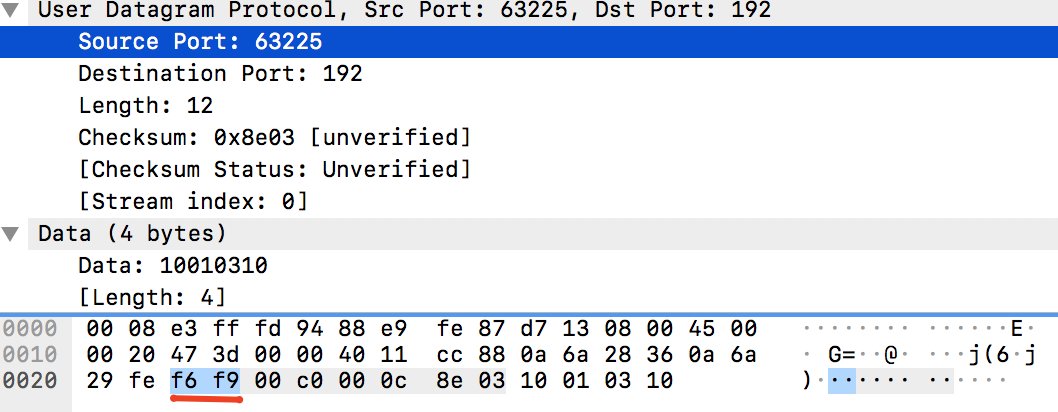
\includegraphics[scale=0.5]{images/UDP2.png}
        \end{itemize}

    \item The value in the length field is the length of what?  Verify your claim with your captured UDP packet
        \begin{itemize}
          \item Similar to how we found the payload in the HTTP lab, the Length value represents the total length of the packet
          \item In Our case it is 8 bytes from the header, and 4 bytes of data, so the Length $=$ 12
          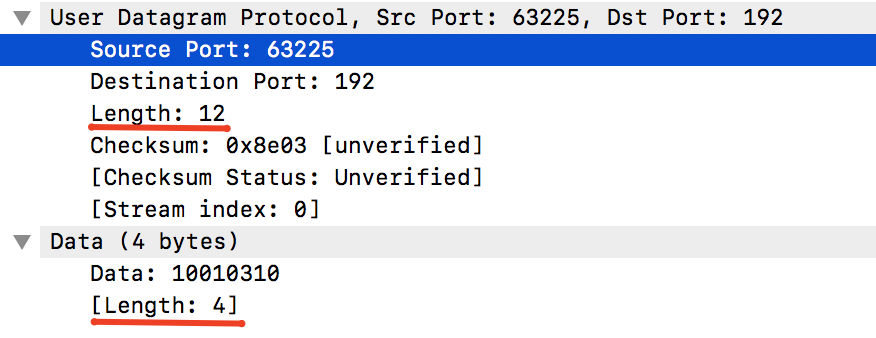
\includegraphics[scale=0.5]{images/UDP3.png}
        \end{itemize}

    \item What is the maximum number of bytes that can be included in a UDP payload?
        \begin{itemize}
          \item the maximum numbere of bytse for a UDP payload is 65535 minus the number of bytes in the header. Which leaves us with (65535 - 8) = 65527 
        \end{itemize}

    \item What is the largest possible source port number?
        \begin{itemize}
          \item Port numbers are 16 bit unsigned integres, 65535 is the maximum port value.
        \end{itemize}

    \item What is the protocol number for UDP?  Give your answer in both hexadecimal and decimal notation
        \begin{itemize}
          \item Decimal: 17
          \item Hexadecimal: 0x11
          \item 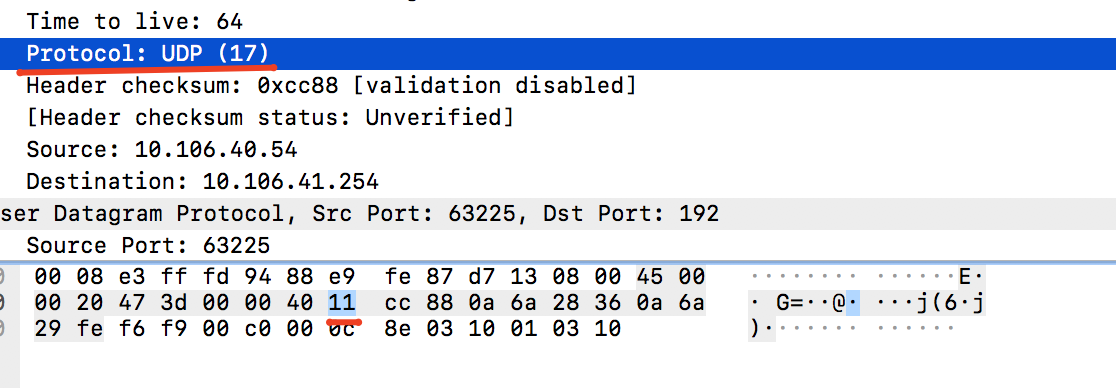
\includegraphics[scale=0.5]{images/UDP7.png}
        \end{itemize}

    \item Examine a pair of UDP packets in which your host sends the first UDP packet and the second UDP packet is a reply to this first UDP packet.  Describe the relationship between
    the port numbers in the two packets.
        \begin{itemize}
          \item As seen earlier with the source and destination ports, the source port of the sent UDP packet will be the destination port of the UDP reply.   
        \end{itemize}
    \end{enumerate}
\end{document}
